\section{Auswertung}
\label{sec:Auswertung}
\subsection{Bestimmung der Zeitkonstante anhand der Aufladekurve}
Um die Aufladekurve des RC-Gliedes zu erhalten, wird der in der Durchführung beschriebene Aufbau betrachtet.
Es ergibt sich das in Abbildung \ref{fig:oz1} dargestellte Bild am Oszillographen, welches die Aufladekurve des betrachteten RC-Gliedes darstellt.

\begin{figure}[H]
  \centering
  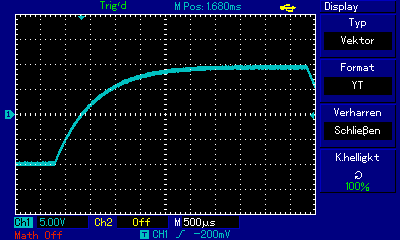
\includegraphics{oz4.png}
  \caption{Aufladekurve des RC-Gliedes.}
  \label{fig:oz1}
\end{figure}

Hierbei ist auf der x-Achse die Zeit $t$ in $\SI{500}{\nano\second}$ pro Kästchen, auf der y-Achse die Kondensatorspannung $U_c$ in $\SI{5}{\volt}$ pro Kästchen aufgetragen.
Um nun eine lineare Ausgleichsrechnung zur Bestimmung der Zeitkonstante $\tau$ durchführen zu können, werden dem Graphen die in Tabelle \ref{tab:werte_a} angegebenen Werte entnommen.


\begin{table}[H]
  \centering
  \caption{Messerte der Aufladekurve des Kondensators.}
  \label{tab:werte_a}
  \sisetup{table-format=1.2}
  \begin{tabular}{c c}
    \toprule
    {$U_c [\si{\milli\second}]$} & {$t [\si{\volt}]$}\\
    \midrule
    \input{build/atabelle.tex}
    \bottomrule
  \end{tabular}
\end{table}

Da sich die Werte wie in \eqref{eqn:gl} angegeben verhalten, kann nicht direkt eine lineare Ausgleichsrechnung durchgeführt werden.
Zuerst müssen die Werte in die Form
\begin{equation}
  U_c' = U_0 \mathrm{e}^{\frac{-t}{RC}}
\end{equation}
gebracht werden.
Dazu wird von den $U_c$ Werten der Wert $U_{\text{end}} = \SI{19.5}{\volt}$ abgezogen sowie das Vorzeichen umgekehrt.
Es ergeben sich hieraus die in Tabelle \ref{tab:werte_a_neu} angegebenen Werte, so dass die Werte $t$ und $\log(U_c')$ an die Funktion
\begin{equation}
  y = m x +b
\end{equation}
gefittet werden können.

\begin{table}[H]
  \centering
  \caption{Veränderte Messwerte der Aufladekurve.}
  \label{tab:werte_a_neu}
  \sisetup{table-format=1.2}
  \begin{tabular}{c c}
    \toprule
    {$U_c [\si{\milli\second}]$} & {$t [\si{\volt}]$}\\
    \midrule
    \input{build/atabelle_neu.tex}
    \bottomrule
  \end{tabular}
\end{table}

Die Ausgleichsrechnung wird durch die Methode der kleinsten Quadrate mit numpy in Python durchgeführt.
Das Ergebnis ist die in Abbildung \ref{fig:plot_a} halblogarithmisch dargestellte Ausgleichsgerade.
Mit
\begin{equation}
  RC = \frac{-1}{m}
\end{equation}
ergibt sich der bestimmte RC-Wert zu
\begin{align}
  a &= \input{build/wert_rc_a.tex}. \\
\end{align}
\begin{figure}[H]
  \centering
  \includegraphics{aplot.pdf}
  \caption{Ausgleichsgerade zur Bestimmung von RC.}
  \label{fig:plot_a}
\end{figure}

\subsection{Messung der Spannungsamplitude und Phasenverschiebung in Abhängigkeit von der Frequenz}

% Tabelle und so hier bla

\subsection{Nutzung des RC-Gliedes zur Integration}
Das RC-Glied wird, wie in der Durchführung beschrieben, zur Integration der angelegten Spannung genutzt.
Dabei wird eine Frequenz von $\nu = \SI{3000}{\hertz}$ verwendet.
Zunächst wird eine Sinusspannung angelegt, so dass
\begin{align}
U_G &= U_0\sin{\omega t}  & U_c &= -\frac{U_0}{\omega}\cos{\omega t}
\end{align}
als Spannungen erwartet werden, wobei $U_G$ die angelegte Spannung, $U_c$ die erwartete Kondensatorspannung und $U_0$ die Amplitude der Sinusspannung bezeichnet.
In Abbildung \ref{fig:sin_r} wird das abgelesene Ergebnis dargestellt.

\begin{figure}[H]
  \centering
  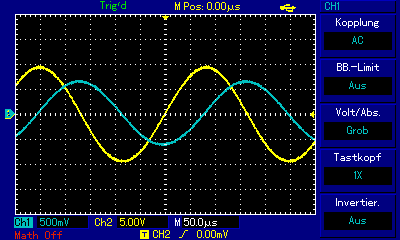
\includegraphics[height=4.5cm]{oz5.png}
  \caption{Erhaltene Kurven für Sinusspannung.}
  \label{fig:sin_r}
\end{figure}


Als nächstes wird die Rechteckspannung überprüft, so dass die Werte
\begin{align}
  U_G &=
  \begin{cases}
    U_0 , &  0 \leq t \leq \frac{T}{2} \\
    -U_0 , & \frac{T}{2} \leq t \leq T
  \end{cases}
   & U_c &=
  \begin{cases}
    at , &  0 \leq t \leq \frac{T}{2} \\
    -at , & \frac{T}{2} \leq t \leq T
  \end{cases}
\end{align}
mit $U_0$ als Amplitude der Rechteckspannung sowie $a$ als positiven Skalierungsfaktor erwartet werden.
Abbildung \ref{fig:rechteck_s} zeigt das am Oszillographen abgelesene Bild.

\begin{figure}[H]
  \centering
  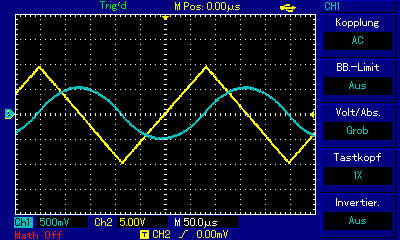
\includegraphics[height=4.5cm]{oz6.png}
  \caption{Erhaltene Kurven für Rechteckspannung.}
  \label{fig:rechteck_s}
\end{figure}

Zum Schluss wird die Dreieckspannung überprüft, woraus sich die erwarteten Werte
\begin{align}
  U_G &=
  \begin{cases}
    at , &  0 \leq t \leq \frac{T}{2} \\
    -at , & \frac{T}{2} \leq t \leq T
  \end{cases}
  & U_c &=
  \begin{cases}
    b t^2 , &  0 \leq t \leq \frac{T}{2} \\
    -b t^2 , & \frac{T}{2} \leq t \leq T
  \end{cases}
\end{align}
mit Skalierungsfaktoren $a$ und $b$ ergeben.
Abbildung \ref{fig:s_s} zeigt das abgelesene Bild.

\begin{figure}[H]
  \centering
  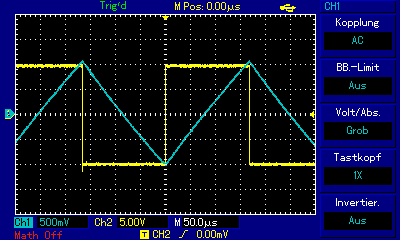
\includegraphics[height=4.5cm]{oz7.png}
  \caption{Erhaltene Kurven für Dreieckspannung.}
  \label{fig:s_s}
\end{figure}
